\documentclass{article}
\usepackage[paperwidth=23.0cm,paperheight=9.5cm,margin=0cm,noheadfoot]{geometry}
\usepackage{amsmath,amssymb}
\usepackage{tikz}
\usetikzlibrary{arrows.meta,positioning,calc,backgrounds}
\usepackage{xcolor}
\usepackage[T1]{fontenc}
\usepackage{lmodern}
\usepackage{tgheros}
\usepackage{sansmath}
\renewcommand{\familydefault}{\sfdefault}
\sansmath
\pagestyle{empty}
\setlength{\parindent}{0pt}

% === Colors ===
\definecolor{deepblue}{HTML}{1A5276}
\definecolor{midblue}{HTML}{2980B9}
\definecolor{lightblue}{HTML}{AED6F1}
\definecolor{lightblue2}{HTML}{D4E6F1}

\definecolor{deeporange}{HTML}{B9470B}
\definecolor{midorange}{HTML}{E67E22}
\definecolor{lightorange}{HTML}{F5CBA7}

\definecolor{deeppurple}{HTML}{6C3483}
\definecolor{midpurple}{HTML}{8E44AD}
\definecolor{lightpurple}{HTML}{D2B4DE}

\definecolor{deepgray}{HTML}{2C3E50}
\definecolor{midgray}{HTML}{7F8C8D}
\definecolor{panelbg}{HTML}{FAFCFE}

\begin{document}
\vspace*{0pt}\noindent
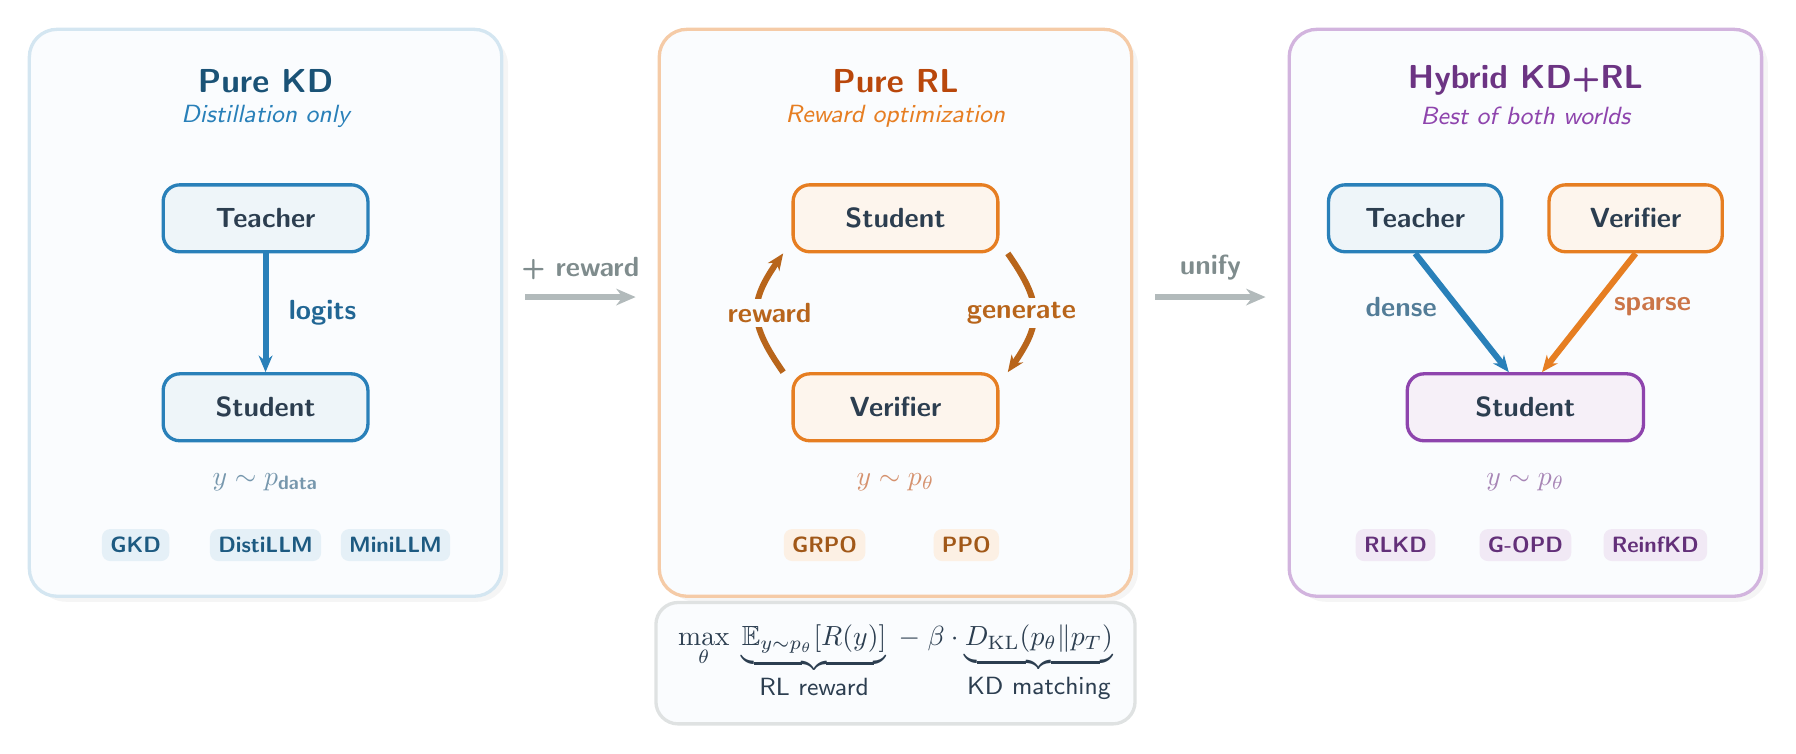
\begin{tikzpicture}[
    >=Stealth,
    entity/.style={
      draw=#1, line width=1.2pt, rounded corners=6pt,
      fill=#1!8,
      font=\normalsize\bfseries, text=deepgray,
      minimum width=2.6cm, minimum height=0.85cm,
      text centered, inner sep=5pt,
    },
    flow/.style={-{Stealth[length=6pt,width=5pt]}, line width=2.2pt, #1},
    pill/.style={
      font=\footnotesize\bfseries, text=#1!70!black,
      fill=#1!12, rounded corners=3pt, inner sep=3pt,
    },
  ]

  % Panel geometry: each 6.0cm wide, gaps 1.5cm for evolution arrows
  % Panel 1: x = 0.5 to 6.5   (center 3.5)
  % Arrow 1:  x = 6.8 to 8.2
  % Panel 2: x = 8.5 to 14.5  (center 11.5)
  % Arrow 2:  x = 14.8 to 16.2
  % Panel 3: x = 16.5 to 22.5 (center 19.5)
  % Total: 23.0 cm

  % =================== Stage 1: Pure KD ===================
  % Shadow
  \fill[black, opacity=0.04, rounded corners=11pt] (0.58, -0.07) rectangle (6.58, 7.13);
  % Background
  \fill[panelbg, rounded corners=10pt] (0.5, 0) rectangle (6.5, 7.2);
  \draw[lightblue2, line width=1.2pt, rounded corners=10pt] (0.5, 0) rectangle (6.5, 7.2);

  % Title
  \node[font=\large\bfseries, deepblue] at (3.5, 6.55) {Pure KD};
  \node[font=\small\itshape, midblue] at (3.5, 6.1) {Distillation only};

  % Teacher → logits → Student
  \node[entity=midblue] (t1) at (3.5, 4.8) {Teacher};
  \node[entity=midblue] (s1) at (3.5, 2.4) {Student};
  \draw[flow=midblue] (t1) -- (s1)
    node[midway, right, font=\normalsize\bfseries, midblue!80!black, xshift=4pt] {logits};

  % Distribution label
  \node[font=\normalsize\bfseries, deepblue!60] at (3.5, 1.45) {$y \sim p_{\text{data}}$};

  % Method pills
  \node[pill=midblue] at (1.85, 0.65) {GKD};
  \node[pill=midblue] at (3.5, 0.65) {DistiLLM};
  \node[pill=midblue] at (5.15, 0.65) {MiniLLM};

  % =================== Evolution arrow 1→2 ===================
  \draw[-{Stealth[length=7pt,width=6pt]}, line width=2.0pt, midgray!60]
    (6.8, 3.8) -- (8.2, 3.8)
    node[midway, above, font=\normalsize\bfseries, midgray, yshift=2pt] {+ reward};

  % =================== Stage 2: Pure RL ===================
  % Shadow
  \fill[black, opacity=0.04, rounded corners=11pt] (8.58, -0.07) rectangle (14.58, 7.13);
  % Background
  \fill[panelbg, rounded corners=10pt] (8.5, 0) rectangle (14.5, 7.2);
  \draw[lightorange, line width=1.2pt, rounded corners=10pt] (8.5, 0) rectangle (14.5, 7.2);

  % Title
  \node[font=\large\bfseries, deeporange] at (11.5, 6.55) {Pure RL};
  \node[font=\small\itshape, midorange] at (11.5, 6.1) {Reward optimization};

  % Student ↔ Verifier with smooth curved arrows
  \node[entity=midorange] (s2) at (11.5, 4.8) {Student};
  \node[entity=midorange] (v2) at (11.5, 2.4) {Verifier};

  % generate: right side arc
  \draw[flow=midorange!80!black] ([xshift=3pt]s2.south east) to[out=-55, in=55, looseness=1.3] ([xshift=3pt]v2.north east);
  \node[font=\normalsize\bfseries, midorange!80!black, fill=panelbg, inner sep=1.5pt] at (13.1, 3.6) {generate};
  % reward: left side arc
  \draw[flow=midorange!80!black] ([xshift=-3pt]v2.north west) to[out=125, in=235, looseness=1.3] ([xshift=-3pt]s2.south west);
  \node[font=\normalsize\bfseries, midorange!80!black, fill=panelbg, inner sep=1.5pt] at (9.9, 3.6) {reward};

  % Distribution label
  \node[font=\normalsize\bfseries, deeporange!60] at (11.5, 1.45) {$y \sim p_\theta$};

  % Method pills
  \node[pill=midorange] at (10.6, 0.65) {GRPO};
  \node[pill=midorange] at (12.4, 0.65) {PPO};

  % =================== Evolution arrow 2→3 ===================
  \draw[-{Stealth[length=7pt,width=6pt]}, line width=2.0pt, midgray!60]
    (14.8, 3.8) -- (16.2, 3.8)
    node[midway, above, font=\normalsize\bfseries, midgray, yshift=2pt] {unify};

  % =================== Stage 3: Hybrid KD+RL ===================
  % Shadow
  \fill[black, opacity=0.04, rounded corners=11pt] (16.58, -0.07) rectangle (22.58, 7.13);
  % Background
  \fill[panelbg, rounded corners=10pt] (16.5, 0) rectangle (22.5, 7.2);
  \draw[lightpurple, line width=1.2pt, rounded corners=10pt] (16.5, 0) rectangle (22.5, 7.2);

  % Title
  \node[font=\large\bfseries, deeppurple] at (19.5, 6.55) {Hybrid KD+RL};
  \node[font=\small\itshape, midpurple] at (19.5, 6.1) {Best of both worlds};

  % Teacher + Verifier → Student
  \node[entity=midblue, minimum width=2.2cm] (t3) at (18.1, 4.8) {Teacher};
  \node[entity=midorange, minimum width=2.2cm] (v3) at (20.9, 4.8) {Verifier};
  \node[entity=midpurple, minimum width=3.0cm] (s3) at (19.5, 2.4) {Student};

  % Dense (blue) and Sparse (orange) arrows
  \draw[flow=midblue] (t3.south) -- ([xshift=-6pt]s3.north)
    node[pos=0.45, left, font=\normalsize\bfseries, deepblue!75, xshift=-3pt] {dense};
  \draw[flow=midorange] (v3.south) -- ([xshift=6pt]s3.north)
    node[pos=0.45, right, font=\normalsize\bfseries, deeporange!75, xshift=3pt] {sparse};

  % Distribution label
  \node[font=\normalsize\bfseries, deeppurple!60] at (19.5, 1.45) {$y \sim p_\theta$};

  % Method pills
  \node[pill=midpurple] at (17.85, 0.65) {RLKD};
  \node[pill=midpurple] at (19.5, 0.65) {G-OPD};
  \node[pill=midpurple] at (21.15, 0.65) {ReinfKD};

  % =================== Bottom equation ===================
  \node[font=\normalsize, deepgray, fill=panelbg, rounded corners=8pt, inner sep=8pt,
        draw=midgray!25, line width=1.2pt]
    at (11.5, -0.85) {
    $\displaystyle \max_\theta \;
    \underbrace{\mathbb{E}_{y \sim p_\theta}[R(y)]}_{\text{\small RL reward}}
    \;-\; \beta \cdot
    \underbrace{D_{\mathrm{KL}}(p_\theta \| p_T)}_{\text{\small KD matching}}$
  };

\end{tikzpicture}
\end{document}
